\documentclass[border=10pt]{standalone}
\usepackage[svgnames]{xcolor}
\usepackage{amsmath}
\usepackage{pgfplots}
\pgfplotsset{compat=newest}
\usepackage[sfdefault]{FiraSans}
\usepackage{FiraMono}
\renewcommand*\familydefault{\sfdefault}
\begin{document}
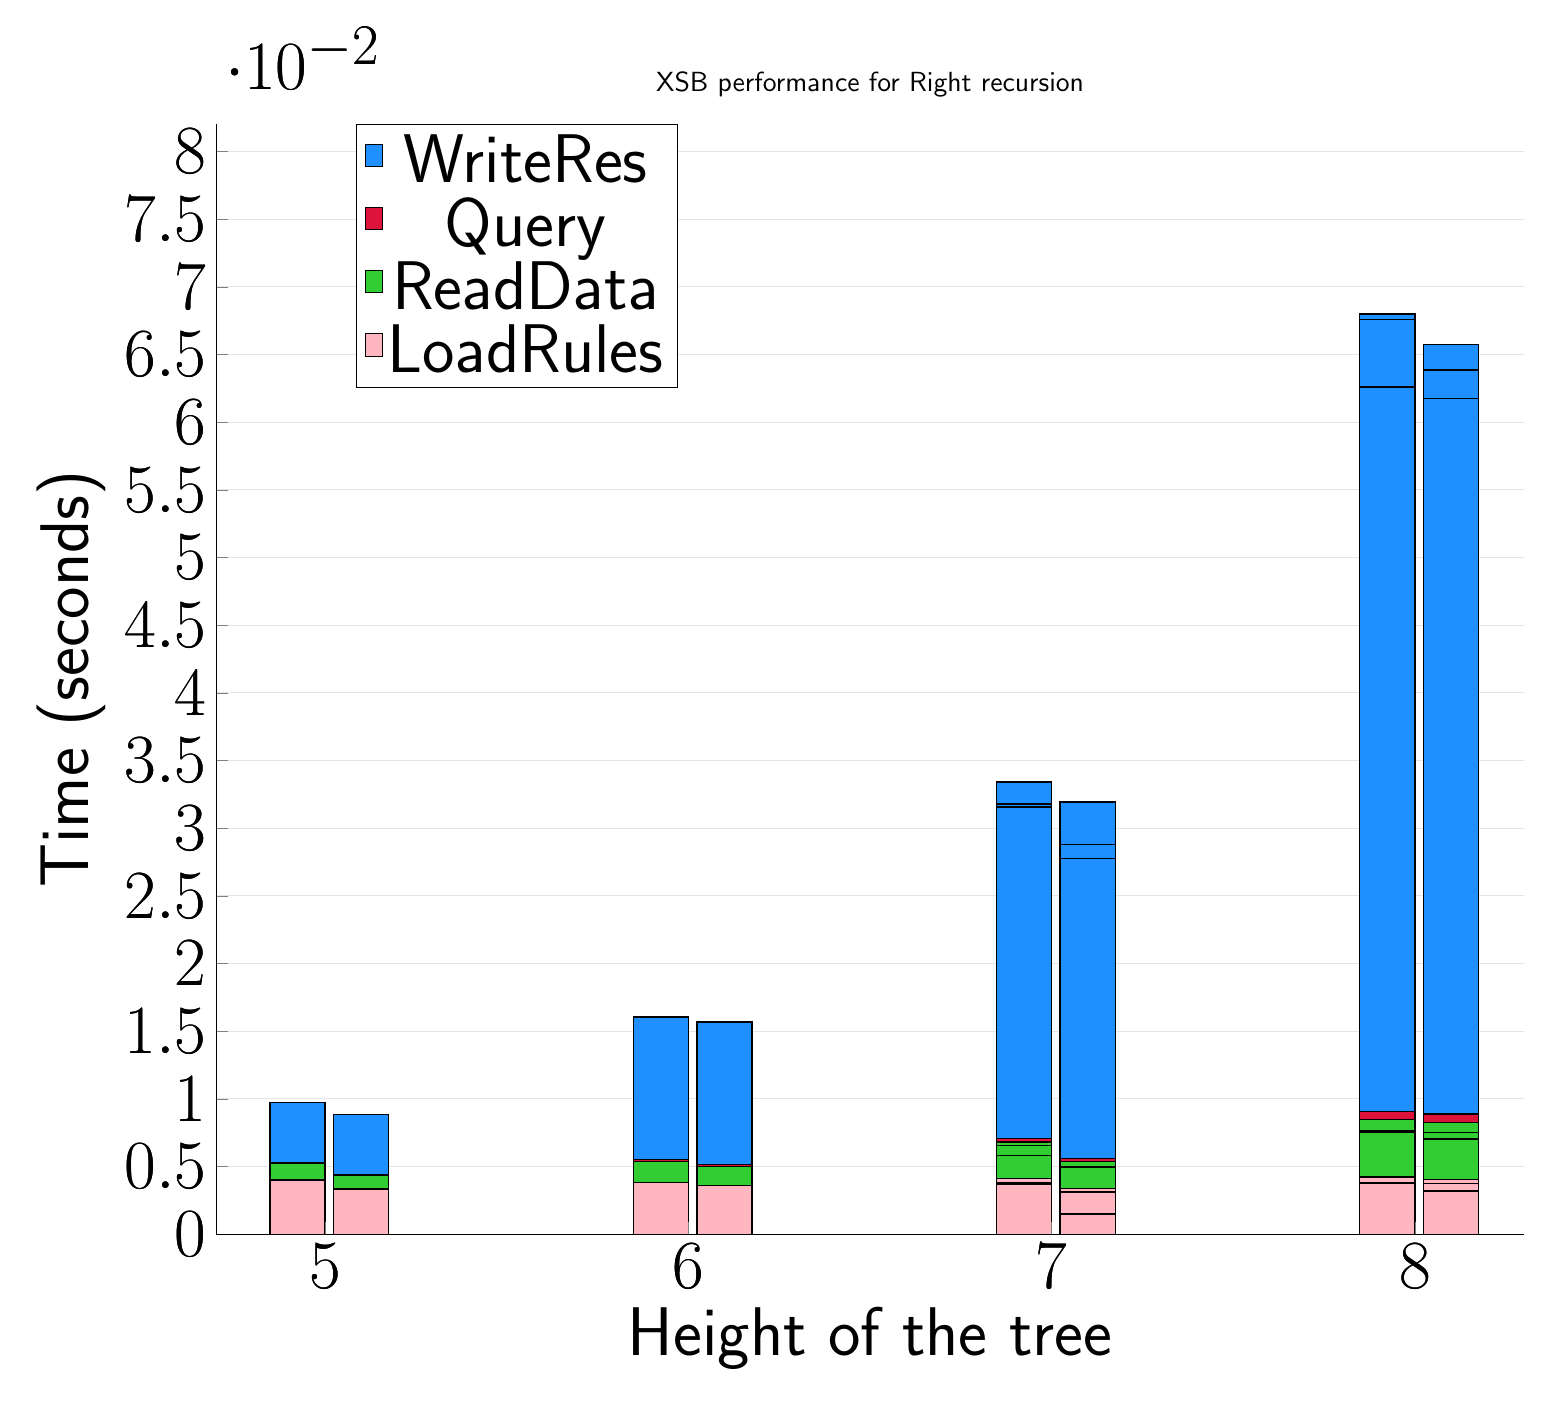
\begin{tikzpicture}
\begin{axis}[
   ybar stacked,
   title={XSB performance for Right recursion},
   bar shift=-10pt,
   width=1.5\textwidth,
   bar width=0.7cm,
   ymajorgrids, tick align=inside,
   major grid style={draw=gray!20},
   xtick=data,
   ymin=0, ymax=0.08207100550333658,
   axis x line*=bottom,
   axis y line*=left,
   enlarge x limits=0.1,
   legend style={
       at={(0.23, 1)},
       anchor=north,
       legend columns=1,
       font=\Huge,
   },
   ylabel={Time (seconds)},
   xlabel={Height of the tree},
   label style={font=\Huge},
   tick label style={font=\Huge},
]
\addlegendimage{fill=DodgerBlue, draw=black, line width=0.2pt}
\addlegendentry{WriteRes}
\addlegendimage{fill=Crimson, draw=black, line width=0.2pt}
\addlegendentry{Query}
\addlegendimage{fill=LimeGreen, draw=black, line width=0.2pt}
\addlegendentry{ReadData}
\addlegendimage{fill=LightPink, draw=black, line width=0.2pt}
\addlegendentry{LoadRules}
\addplot +[fill=LightPink, draw=black, line width=0.5pt] coordinates {
    (5, 0.004019578297932943)
    (6, 0.003815333048502603)
    (7, 0.0037929217020670563)
    (7, 0.004097064336140949)
    (7, 0.0036546389261881535)
    (8, 0.0037880738576253265)
    (8, 0.0037890275319417293)
    (8, 0.0042193730672200535)
};
\addplot +[fill=LimeGreen, draw=black, line width=0.5pt] coordinates {
    (5, 0.0012047290802001968)
    (6, 0.0015676816304524765)
    (7, 0.003025293350219723)
    (7, 0.00247995058695475)
    (7, 0.0021464029947916665)
    (8, 0.0037619272867838566)
    (8, 0.0038452943166097)
    (8, 0.004238287607828777)
};
\addplot +[fill=Crimson, draw=black, line width=0.5pt] coordinates {
    (5, 6.429354349772137e-05)
    (6, 0.000160376230875651)
    (7, 0.000266075134277344)
    (7, 0.0002660751342773437)
    (7, 0.00025502840677897137)
    (8, 0.0005280176798502603)
    (8, 0.0007113615671793619)
    (8, 0.0006190141042073566)
};
\addplot +[fill=DodgerBlue, draw=black, line width=0.5pt] coordinates {
    (5, 0.004445393880208335)
    (6, 0.010506868362426777)
    (7, 0.02470239003499349)
    (7, 0.02473290761311849)
    (7, 0.02735336621602373)
    (8, 0.054512580235799135)
    (8, 0.05965391794840494)
    (8, 0.05850068728129068)
};
\end{axis}
\begin{axis}[
   ybar stacked,
   bar shift=13pt,
   width=1.5\textwidth,
   bar width=0.7cm,
   ymajorgrids, tick align=inside,
   major grid style={draw=none},
   xtick=data,
   ymin=0, ymax=0.08207100550333658,
   axis x line*=none,
   axis y line*=none,
   enlarge x limits=0.1,
   label style={font=\Huge},
   tick label style={font=\Huge},
]
\addplot +[fill=LightPink, draw=black, line width=0.5pt] coordinates {
    (5, 0.0033443333333333333)
    (6, 0.0036093333333333338)
    (7, 0.0014883333333333335)
    (7, 0.003356333333333333)
    (7, 0.003124333333333333)
    (8, 0.0037563333333333303)
    (8, 0.0032073333333333333)
    (8, 0.004022666666666663)
};
\addplot +[fill=LimeGreen, draw=black, line width=0.5pt] coordinates {
    (5, 0.0010013333333333341)
    (6, 0.0013993333333333334)
    (7, 0.0016370000000000002)
    (7, 0.0020286666666666634)
    (7, 0.0018419999999999999)
    (8, 0.0037633333333333334)
    (8, 0.0038220000000000003)
    (8, 0.0042309999999999995)
};
\addplot +[fill=Crimson, draw=black, line width=0.5pt] coordinates {
    (5, 5.2333333333334766e-05)
    (6, 0.00013566666666666363)
    (7, 0.00012766666666666701)
    (7, 0.000217666666666667)
    (7, 0.00021700000000000167)
    (8, 0.0005273333333333333)
    (8, 0.0007116666666666683)
    (8, 0.0006200000000000027)
};
\addplot +[fill=DodgerBlue, draw=black, line width=0.5pt] coordinates {
    (5, 0.004448999999999998)
    (6, 0.010534333333333335)
    (7, 0.024505)
    (7, 0.023188333333333328)
    (7, 0.02675633333333333)
    (8, 0.05370666666666666)
    (8, 0.056115)
    (8, 0.056848333333333334)
};
\end{axis}
\end{tikzpicture}

\end{document}
